\chapter{Ewaluacja}
\label{cha:ewaluacja}
Rozdział prezentuje działanie aplikacji na przykładzie procesu obliczania kwoty ubezpieczenia samochodowego. Przedstawione zostały wybrane najważniejsze funkcjonalności systemu.

%---------------------------------------------------------------------------
\section{Model ARD}
\label{sec:modelARD}
Przykład, na którym zostanie zaprezentowana aplikacja, obrazuje proces związany z~obliczaniem kwoty płatności na rzecz ubezpieczenia samochodowego. Jak wiadomo kwota takiego ubezpieczenia zależy od wielu zmiennych, takich jak liczba wypadków, wiek kierowcy czy rodzaj samochodu. Rysunek~\ref{fig:ardInsuranceExample} prezentuje diagram \emph{ARD}, który mógłby zostać stworzony przez analityka biznesowego, jako prototyp takiego procesu.
\begin{figure}
    \centering
    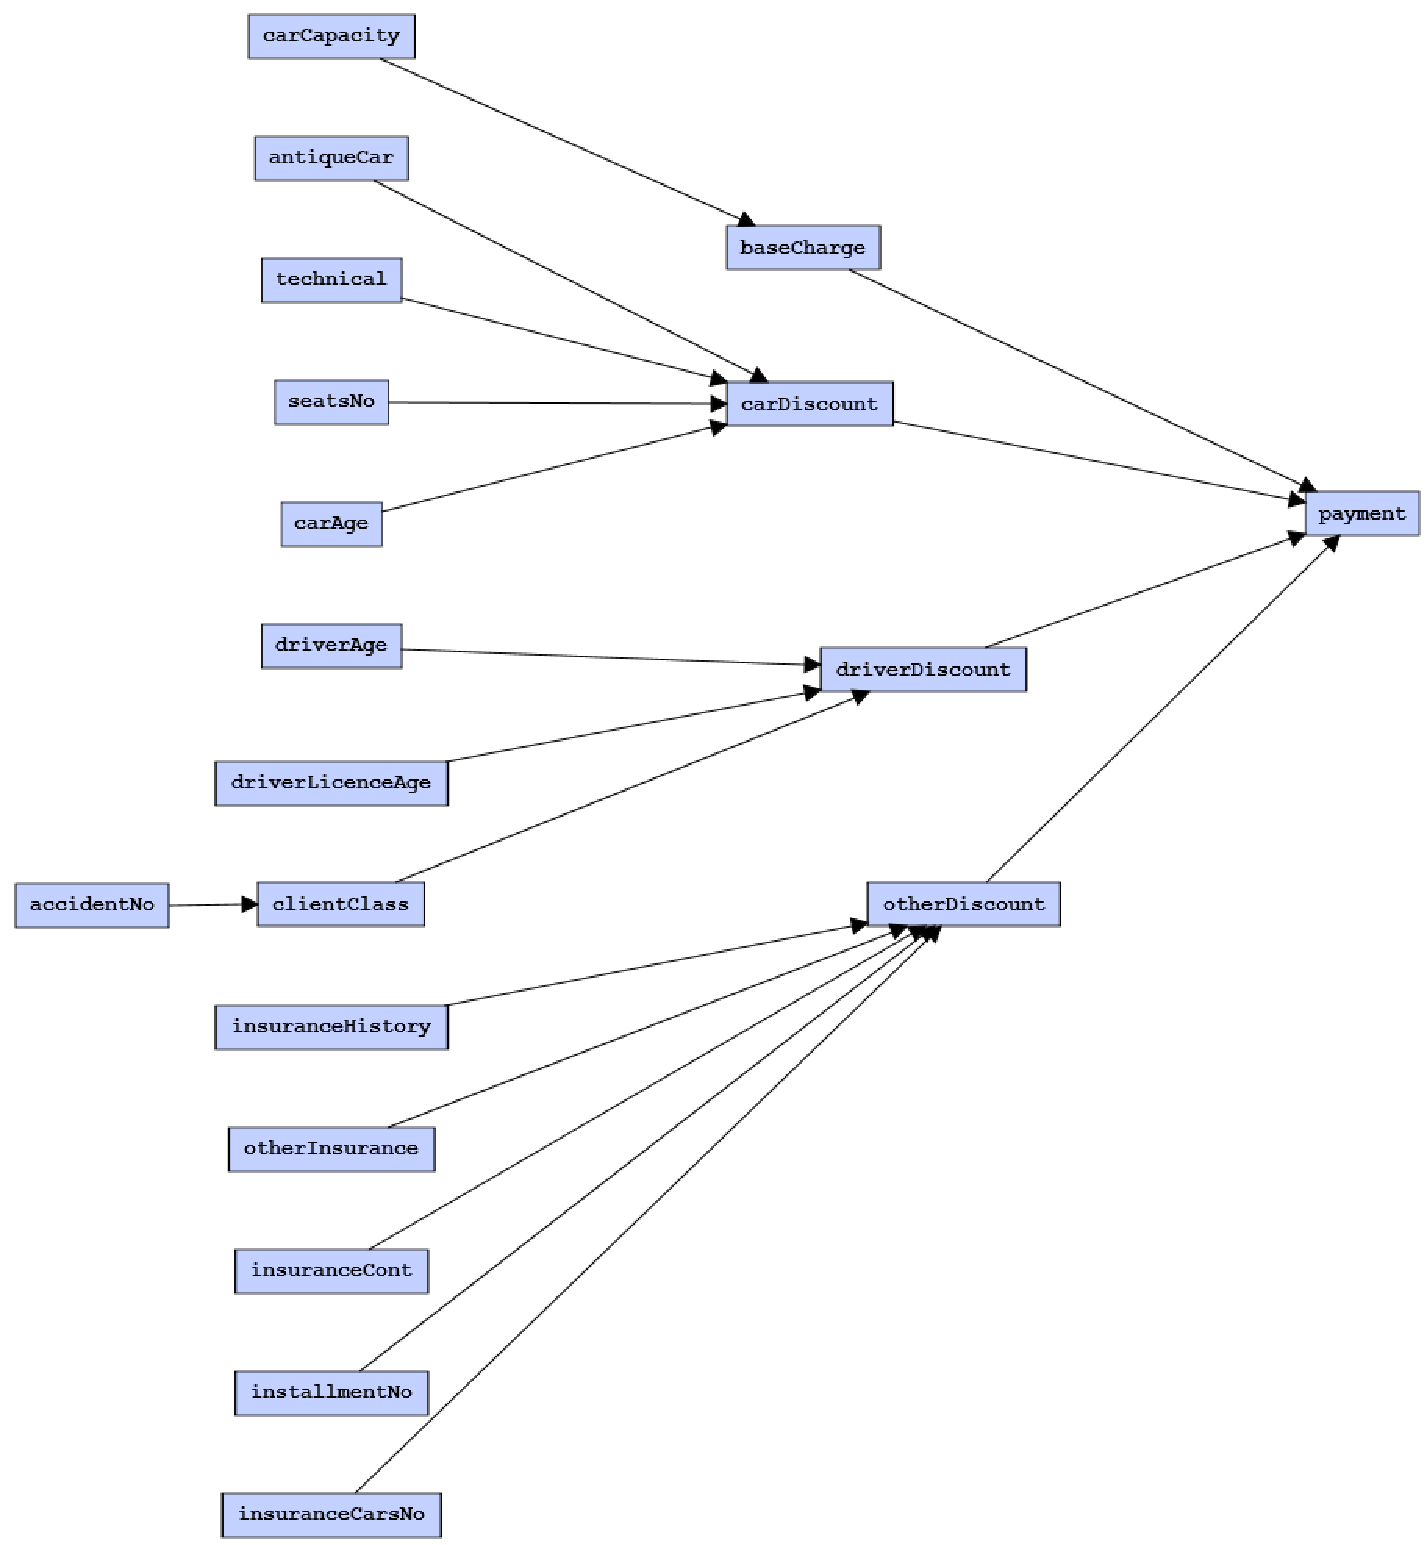
\includegraphics[width=\textwidth]{./assets/ardInsuranceExample.pdf}
    \caption{Diagram \emph{ARD} będący prototypem procesu obliczania kwoty ubezpieczenia samochodowego. Przykład opracowany na bazie studium przypadku przygotowanego w~ramach ewaluacji metodyki Semantycznia Inżynieria Wiedzy~\cite{gjn2011hab}}
    \label{fig:ardInsuranceExample}
\end{figure} 
Tabela~\ref{tab:att} opisuje wszystkie własności, przedstawione na diagramie \emph{ARD} (rysunek~\ref{fig:ardInsuranceExample}). Podany jest ich typ, zakres oraz krótki opis.
\begin{table}
    \begin{tabular}{|p{3.6cm}|p{1.4cm}|p{1.8cm}|p{7cm}|}
    %\cline{1-5}
    \hline
    \textbf{~nazwa~} & \textbf{~typ~} & \textbf{~zakres~} & \textbf{~opis~}\\ \hline\hline
    \texttt{accidentNo} & integer & [0;inf] & liczba kolizji spowodowanych w~okresie ostatnich 12 miesięcy\\ \hline
    \texttt{clientClass} & integer & [-1;9] & klasa jaką posiada klient\\ \hline
    \texttt{carCapacity} & integer & [0;inf] & pojemność silnika [$cm^{3}$]\\ \hline
    \texttt{baseCharge} & integer & [0;inf] & stawka podstawowa w~[$PLN$]\\ \hline
    \texttt{driverAge} & integer & [16;inf] & wiek właściciela pojazdu\\ \hline
    \texttt{driverLicenseAge} & integer & [0;inf] & okres posiadania prawa jazdy przez właściciela pojazdu \\ \hline
    \texttt{driverDiscount} & integer & --- & suma zniżek \texttt{driverAge} i~\texttt{drLicAge} \\ \hline
    \texttt{carAge} & integer & [0;inf] & wiek samochodu\\ \hline
    \texttt{antiqueCar} & boolean & [true; false] & pojazd historyczny \\ \hline
    \texttt{seatsNo} & integer & [2;9] & liczba siedzeń w~pojeździe \\ \hline
    \texttt{technical} & boolean & [true; false] & aktualne badania techniczne\\ \hline
    \texttt{carDiscount} & integer & --- & suma zniżek za \texttt{carAge}, \texttt{historiCar}, \newline \texttt{noSeats} i~\texttt{technical}\\ \hline
    \texttt{installmentNo} & integer & [1;2] & liczba rat \\ \hline
    \texttt{insuranceCont} & boolean & [true; false] & kontynuacja ubezpieczenia \\ \hline
    \texttt{insuranceCarsNo} & integer & [0;inf] & liczba ubezpieczonych samochodów\\ \hline
    \texttt{otherInsurance} & boolean & [true; false] & inne ubezpieczenia\\ \hline
    \texttt{insuranceHistory} & integer & [0;inf] & historia ubezpieczenia \\ \hline
    \texttt{otherDiscount} & integer & --- & suma zniżek za \texttt{noRates}, \texttt{contIns}, \newline \texttt{noCarsIns}, \texttt{otherIns}, \texttt{insHistory} \\ \hline
    \texttt{payment} & float & [0;inf] & ostateczna opłata za ubezpiecznie danego pojazdu w~[$PLN$]\\ \hline
    \end{tabular}\vspace{-2mm}
       \caption{Opis własności w~prototypie procesu obliczania kwoty ubezpieczenia samochodowego. Przykład opracowany na bazie studium przypadku przygotowanego w~ramach ewaluacji metodyki Semantycznia Inżynieria Wiedzy~\cite{gjn2011hab} }
       \label{tab:att}
    \vspace{-3mm}
\end{table} 
Na tej podstawie stworzony został plik \emph{HML}. Zawartość pliku, ze względu na spory rozmiar, nie jest tutaj wylistowana.


%---------------------------------------------------------------------------
\section{Interfejs użytkownika}
\label{sec:interfejsUżytkownika}
Po uruchomieniu aplikacji pierwszym widokiem, z~którym ma do czynienia użytkownik jest domyślny ekran z~omawianego w~rozdziale~\ref{cha:projektAplikacji} komponentu \emph{Home}, co prezentuje rysunek~\ref{fig:darHome}.
\begin{figure}
    \centering
    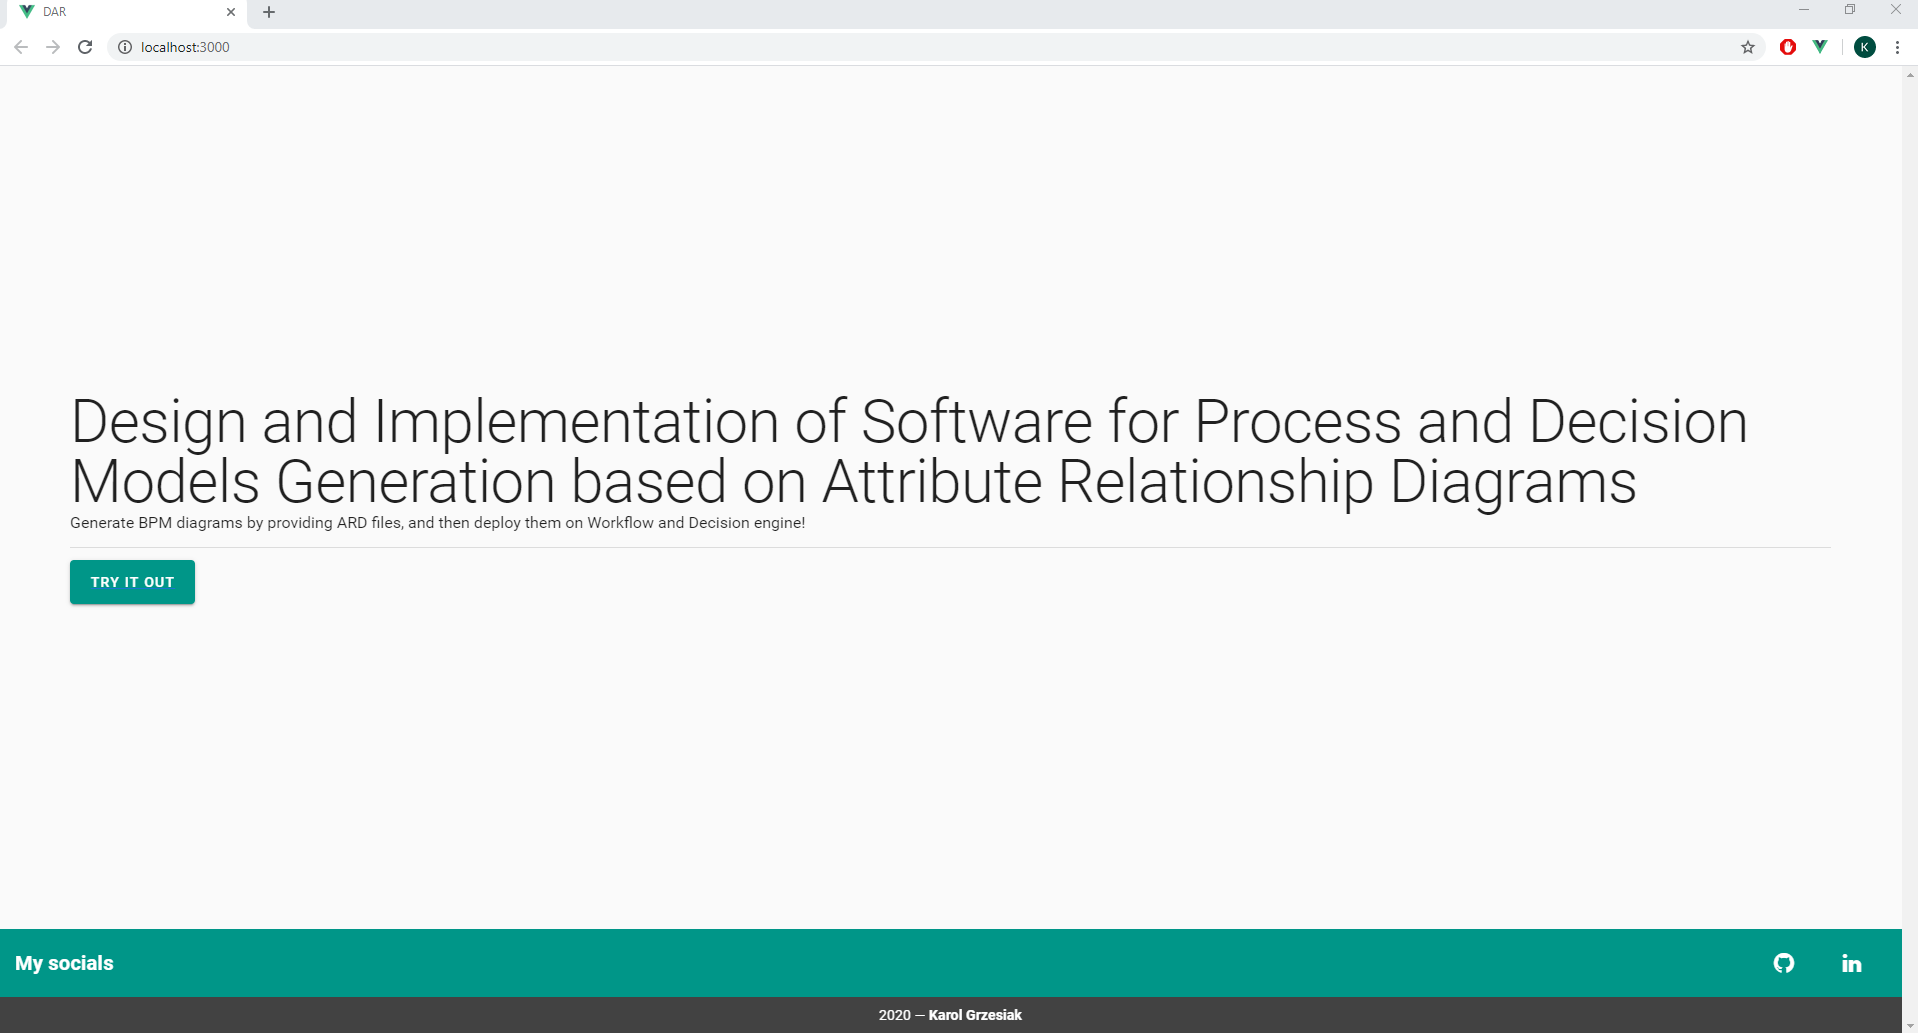
\includegraphics[width=\textwidth]{./assets/darHome.png}
    \caption{Domyślny ekran aplikacji ,,DAR''}
    \label{fig:darHome}
\end{figure} 

Po naciśnięciu przycisku ,,TRY IT OUT'', użytkownik zostaje przeniesiony do głównej części interfejsu użytkownika, czyli do widoku z~komponentu \emph{HML}. W tym miejscu prezentowane są wszystkie pliki \emph{HML}, z~których informacje znajdują się w~bazie danych. Użytkownik ma możliwość dodania nowego pliku, a~także wykonania akcji na plikach już dodanych. W przypadku naciśnięcia na któryś z~wyświetlanych plików, aplikacja prezentuje dwa przyciski: ,,DEPLOY'' oraz ,,DELETE''. Naciśnięcie pierwszego przycisku powoduje generację modeli \emph{BPMN} oraz \emph{DMN}, a~następnie wdrożenie ich na platformę \emph{Camunda}, aby finalnie przenieść użytkownika na wspomnianą platformę. Naciśnięcie drugiego przycisku powoduje usunięcie pliku z~bazy danych. Rysunek~\ref{fig:darHML} przedstawia opisany interfejs po wgraniu dwóch plików \emph{HML}. Plik ,,example'' to plik zawierający wcześniej opisywany model \emph{ARD}. Dalsza część rozdziału opisuję scenariusz, w~którym naciśnięty zostaje zielony przycisk pod plikiem ,,example'' i~plik zostaje wdrożony.  
\begin{figure}
    \centering
    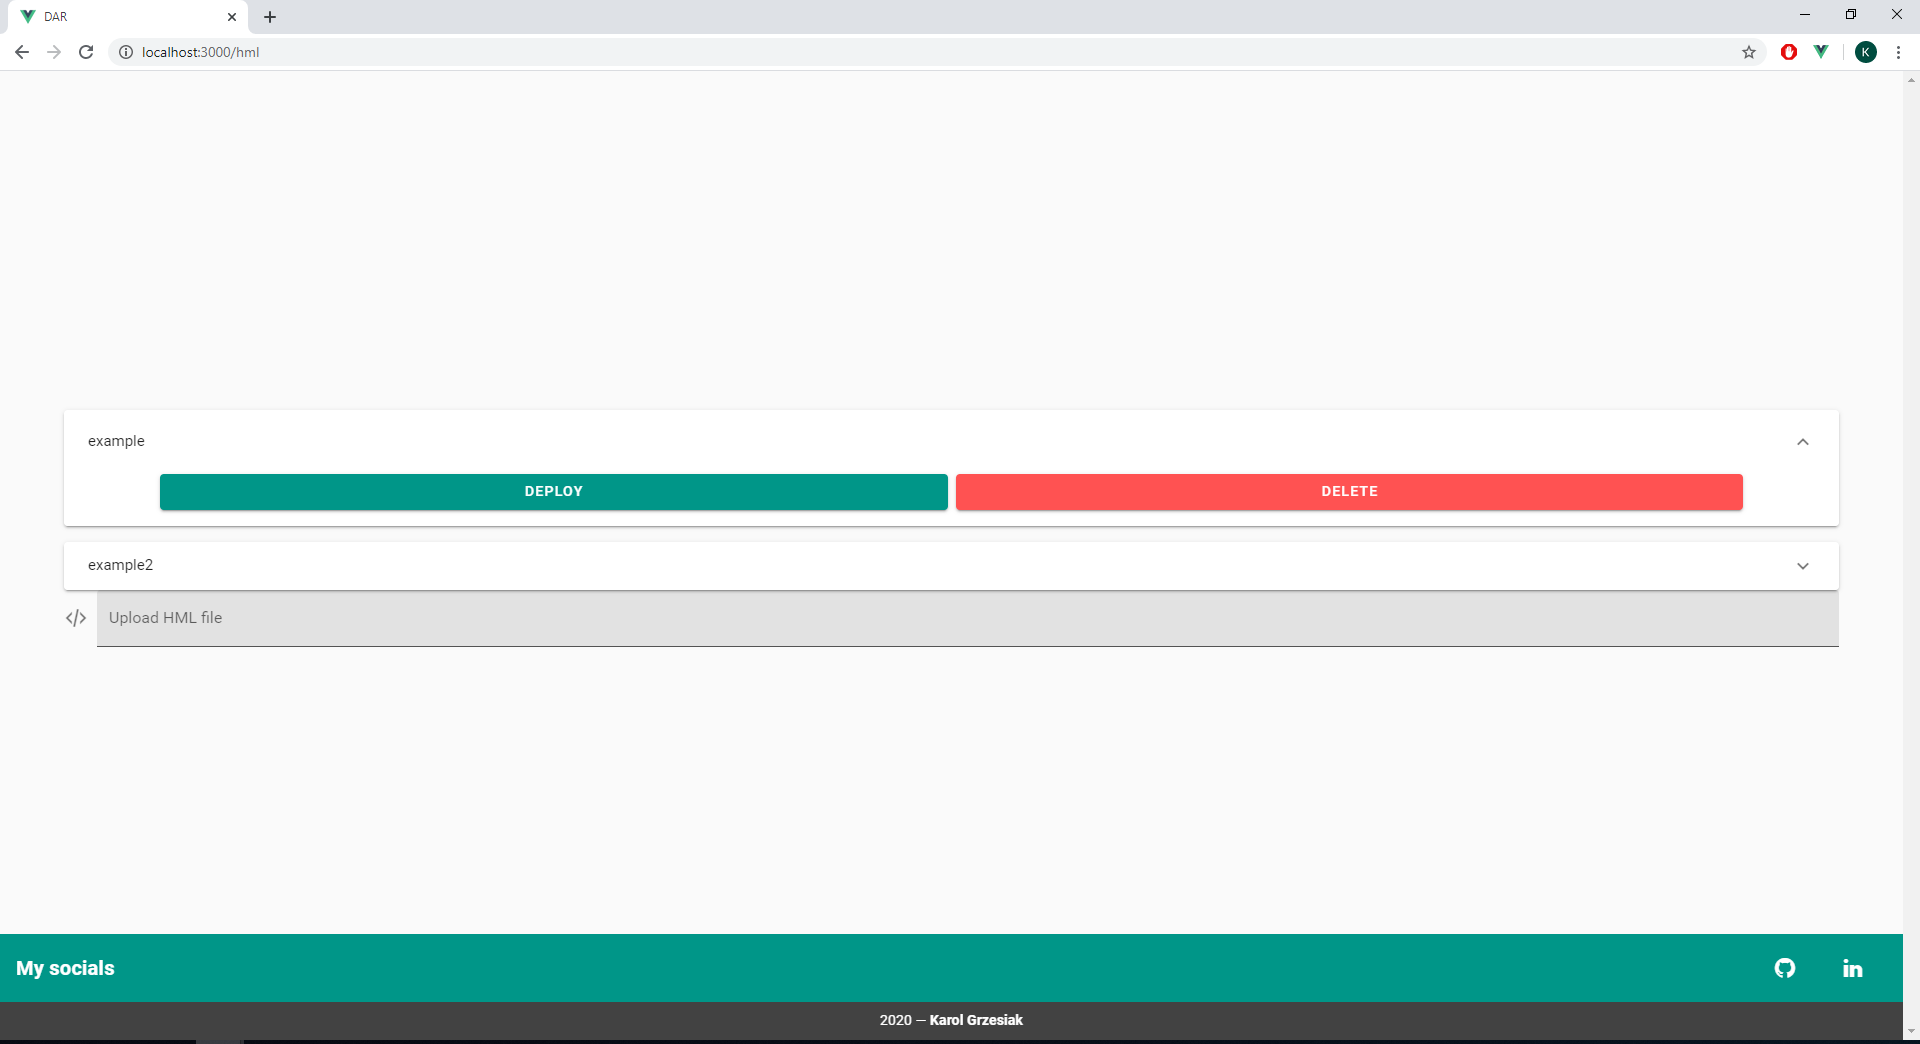
\includegraphics[width=\textwidth]{./assets/darHML.png}
    \caption{Główny ekran interfejsu użytkownika aplikacji ,,DAR''}
    \label{fig:darHML}
\end{figure}

%---------------------------------------------------------------------------
\section{Camunda}
\label{sec:camunda}
Po wdrożeniu pliku zawierającego model opisany w~podrozdziale~\ref{sec:modelARD} użytkownik zostaje przeniesiony na platformę \emph{Camunda}. Domyślny widok, który zostaje mu zaprezentowany przedstawia rysunek~\ref{fig:camundaDefault}. Do dyspozycji są trzy aplikacje, najważniejsze z nich to \emph{Camunda Cockpit} oraz \emph{Camunda Tasklist}. Były one opisywane w~rozdziale~\ref{sec:zewnętrznySystem}.
\begin{figure}
    \centering
    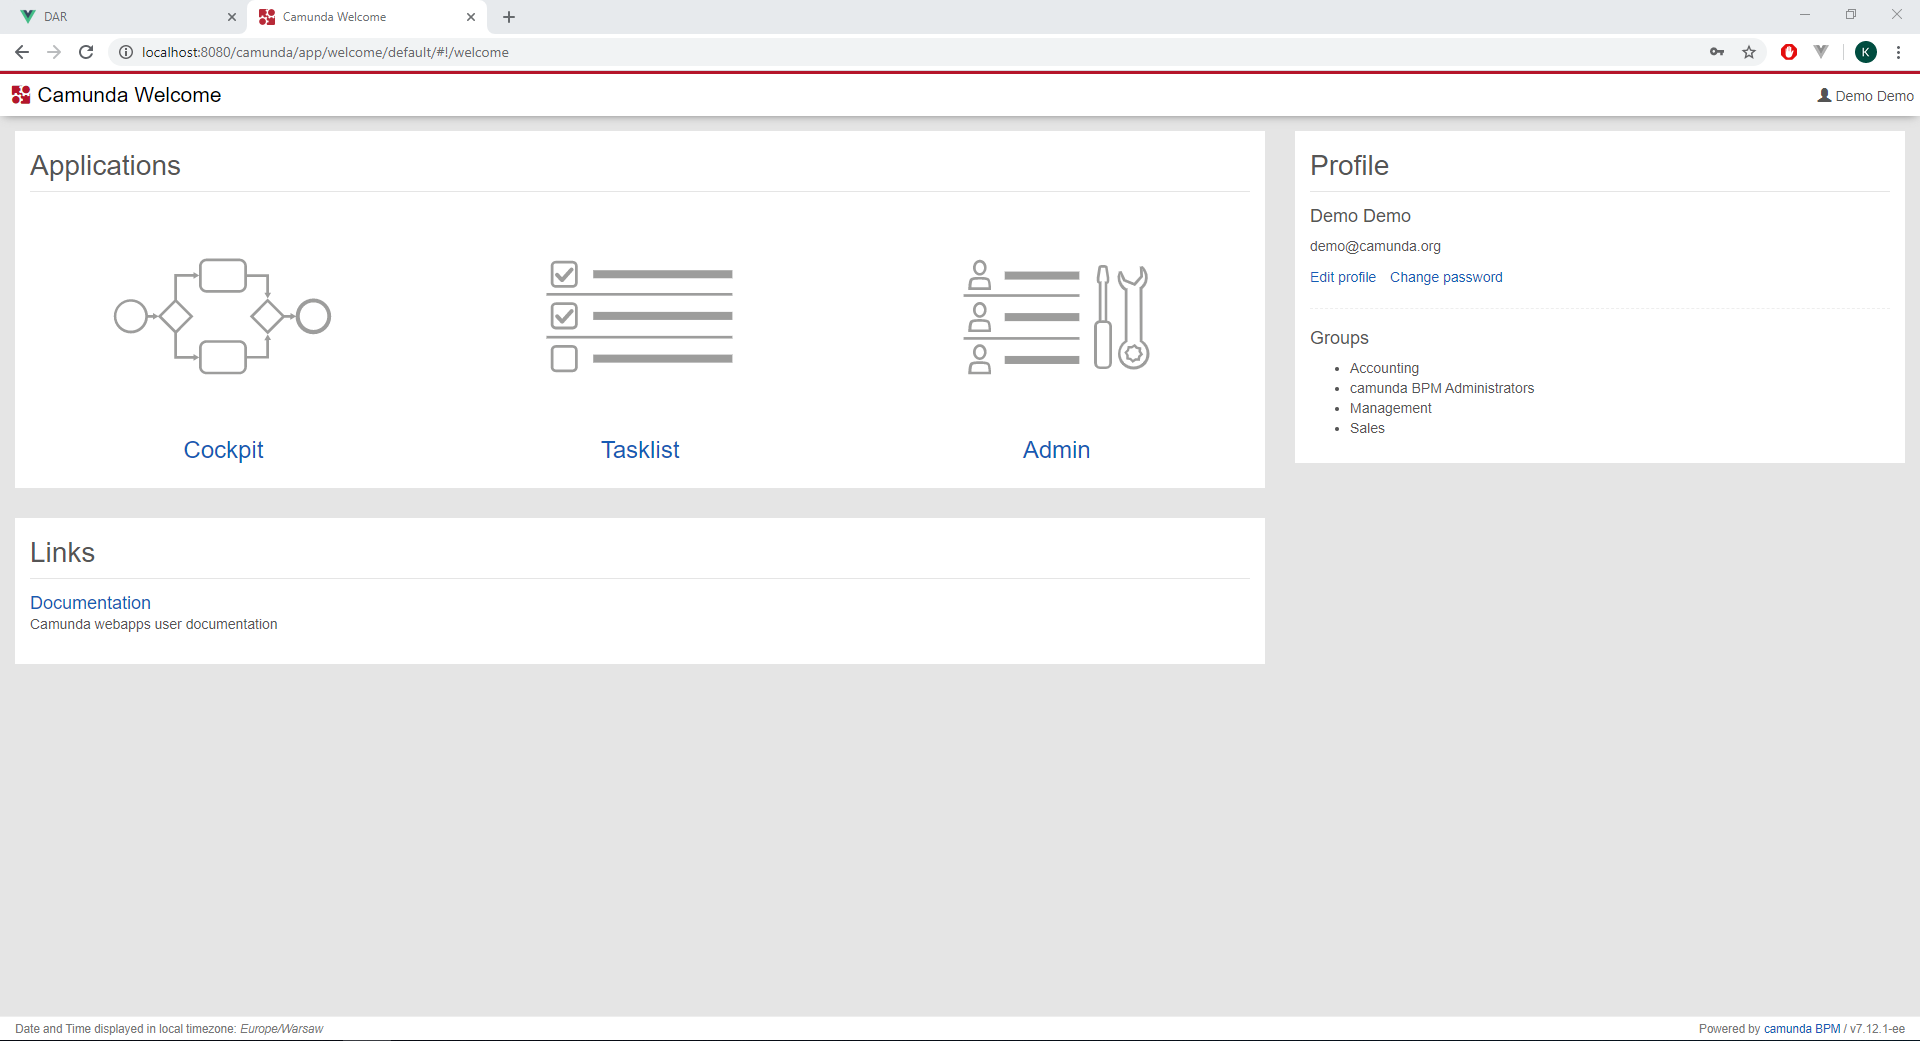
\includegraphics[width=\textwidth]{./assets/camundaDefault.png}
    \caption{Domyślny ekran platformy \emph{Camunda} po wdrożeniu pliku \emph{HML}}
    \label{fig:camundaDefault}
\end{figure}

Rysunek~\ref{fig:camundaCockpitDefault} przedstawia domyślny ekran aplikacji \emph{Camunda Cockpit}. Znajduje się na nim wiele metryk służących do analizy działań na platformie oraz informację o uruchomionych procesach.
\begin{figure}
    \centering
    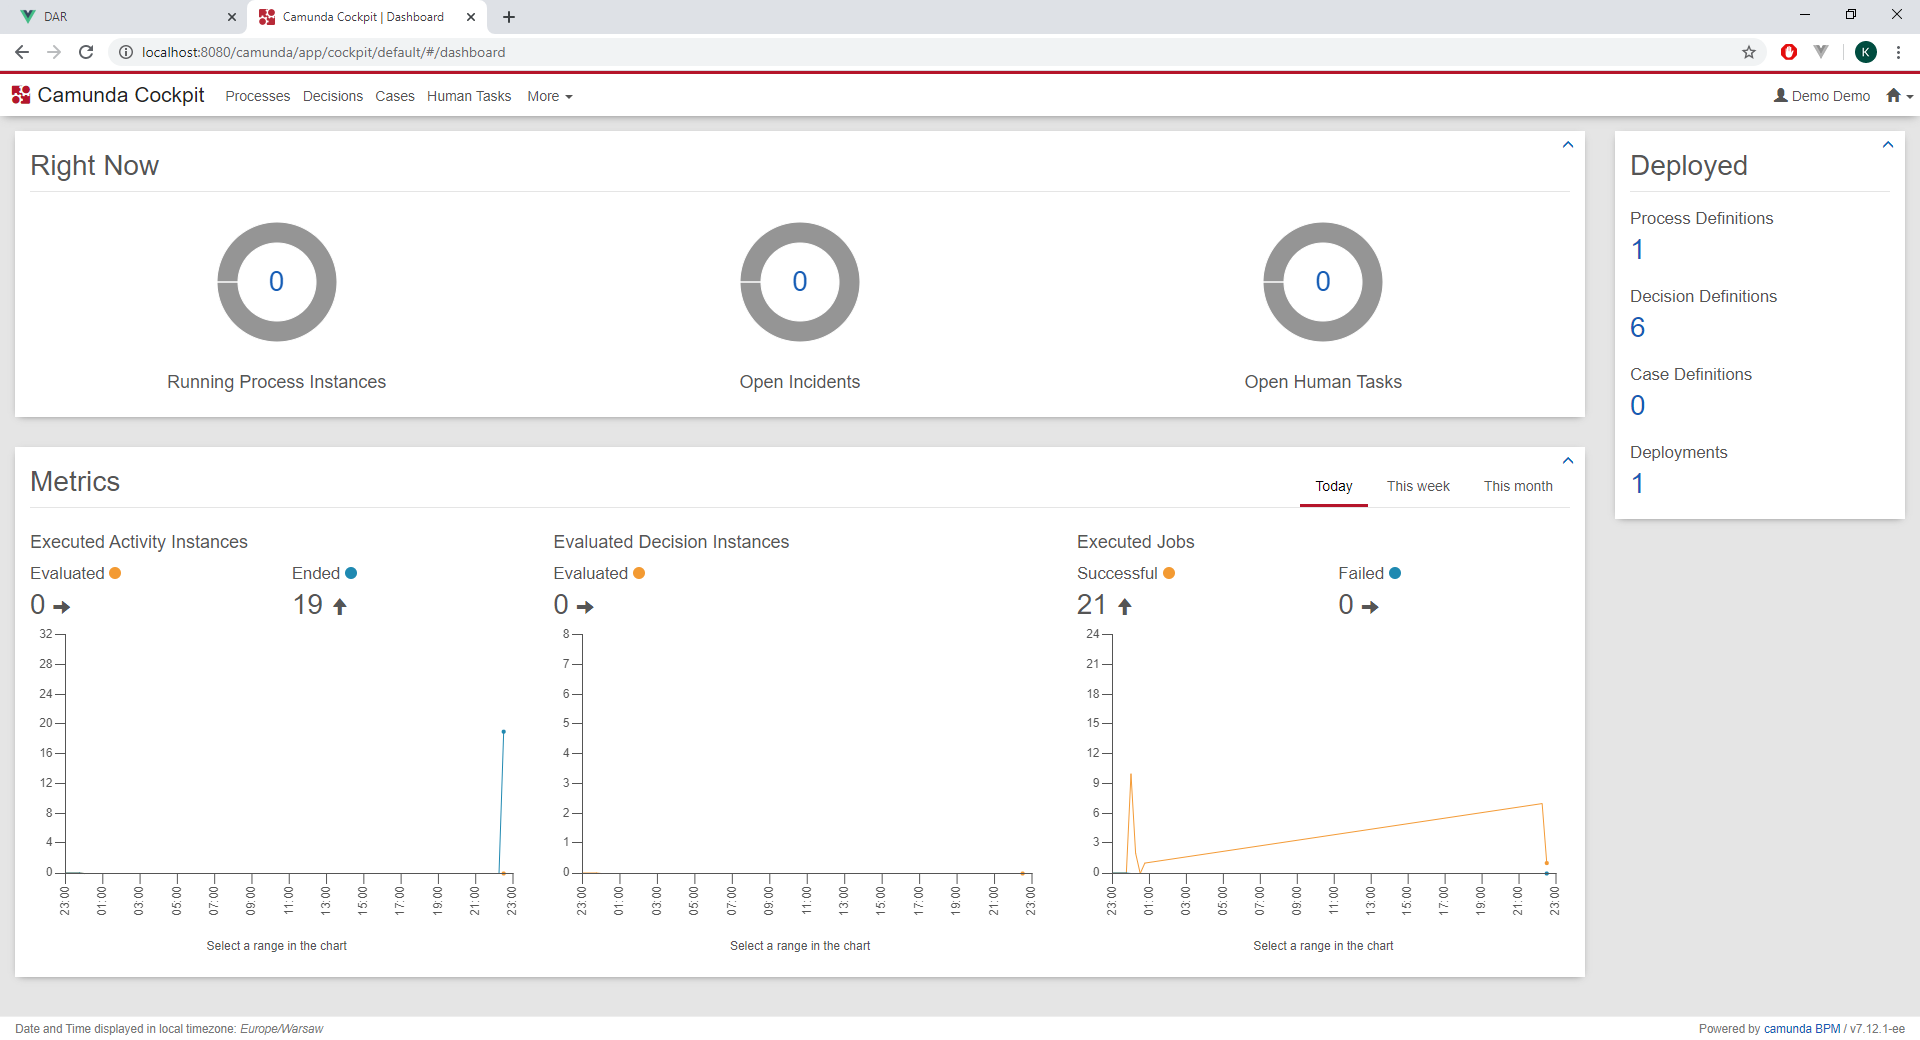
\includegraphics[width=\textwidth]{./assets/camundaCockpitDefault.png}
    \caption{Domyślny ekran \emph{Camunda Cockpit}}
    \label{fig:camundaCockpitDefault}
\end{figure}
Przechodząc do zakładki ,,Deployments'' (,,More`` $\rightarrow$ ,,Deployments``) prezentowane są wszystkie wdrożenia, które miały miejsce. Jak widać na rysunku~\ref{fig:camundaCockpitDeployments} pojawiło się tutaj wdrożenie pliku ,,example'', a~wraz z~nim wygenerowane modele w~notacjach \emph{BPMN} oraz \emph{DMN}. Rysunki~\ref{fig:camundaExampleBPMN} oraz~\ref{fig:camundaExampleDMN} prezentują stworzone wspomniane modele.
\begin{figure}
    \centering
    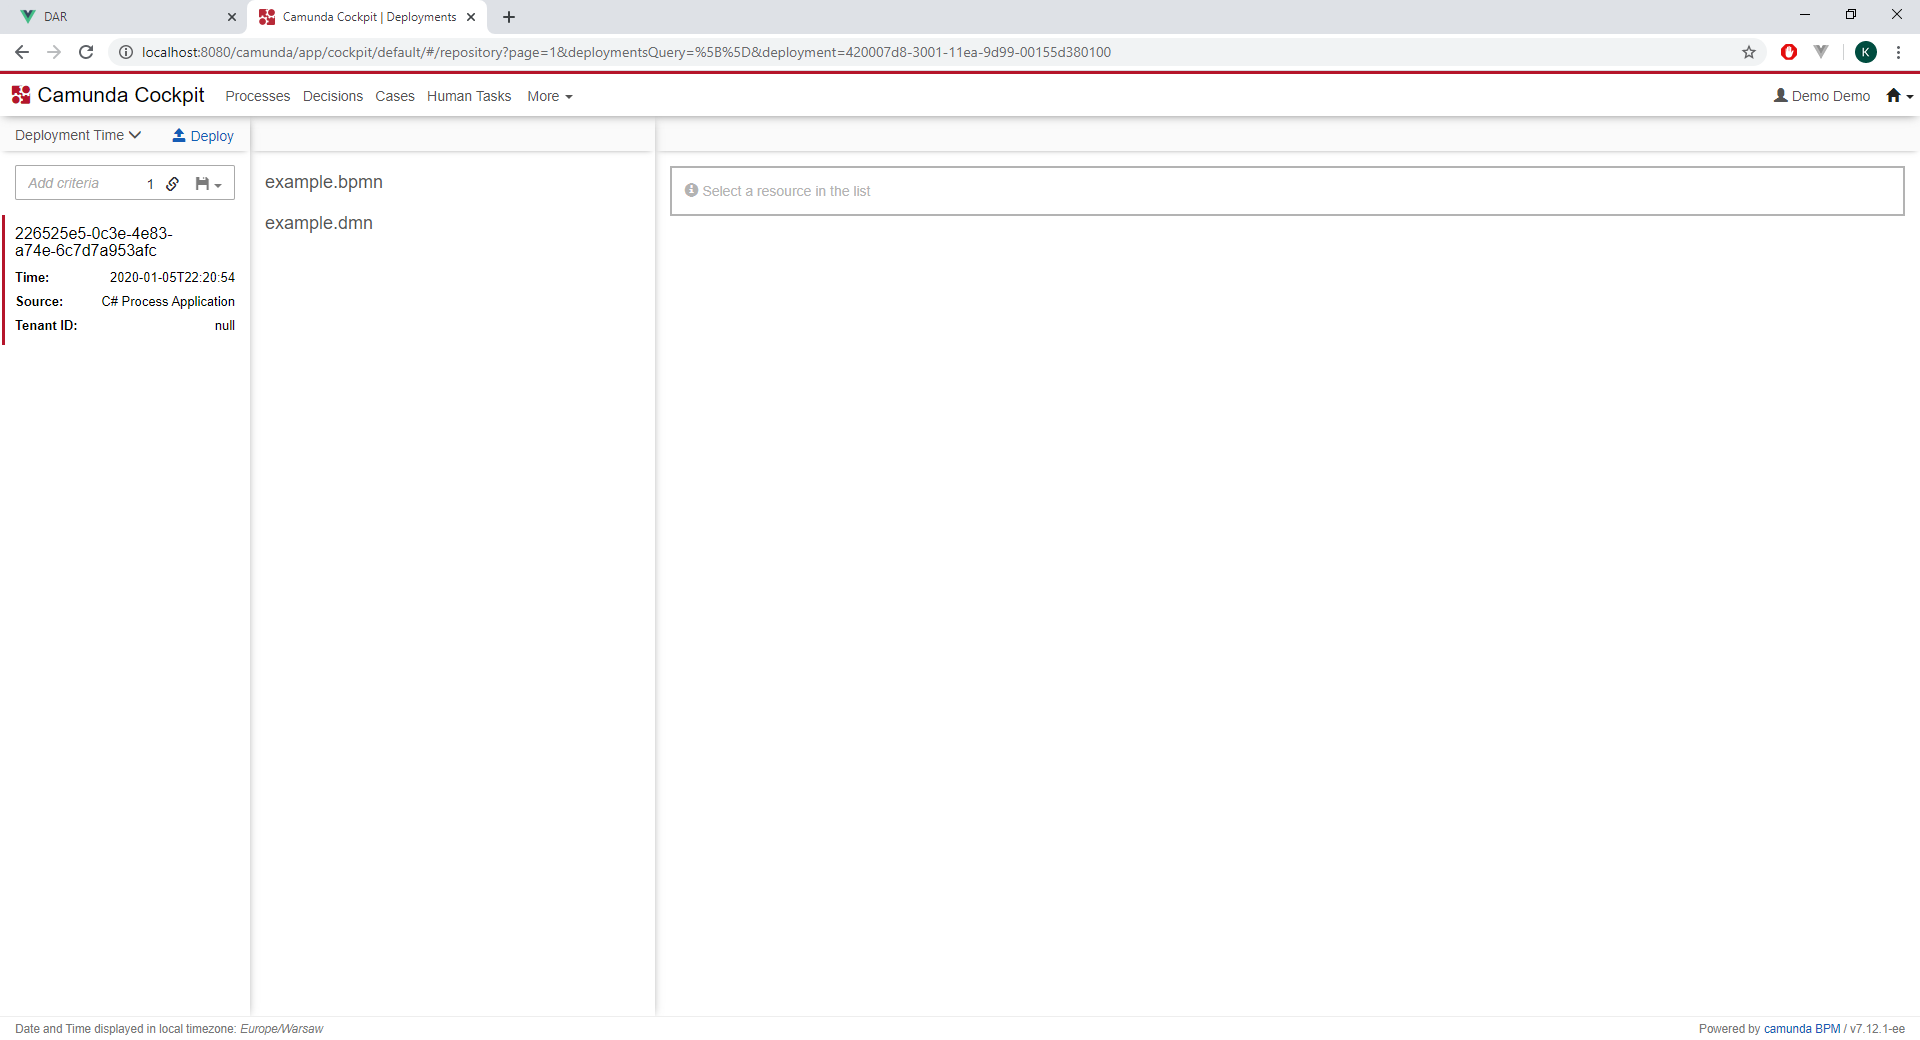
\includegraphics[width=\textwidth]{./assets/camundaCockpitDeployments.png}
    \caption{Ekran wdrożeń \emph{Camunda Cockpit}}
    \label{fig:camundaCockpitDeployments}
\end{figure}
\begin{figure}
    \centering
    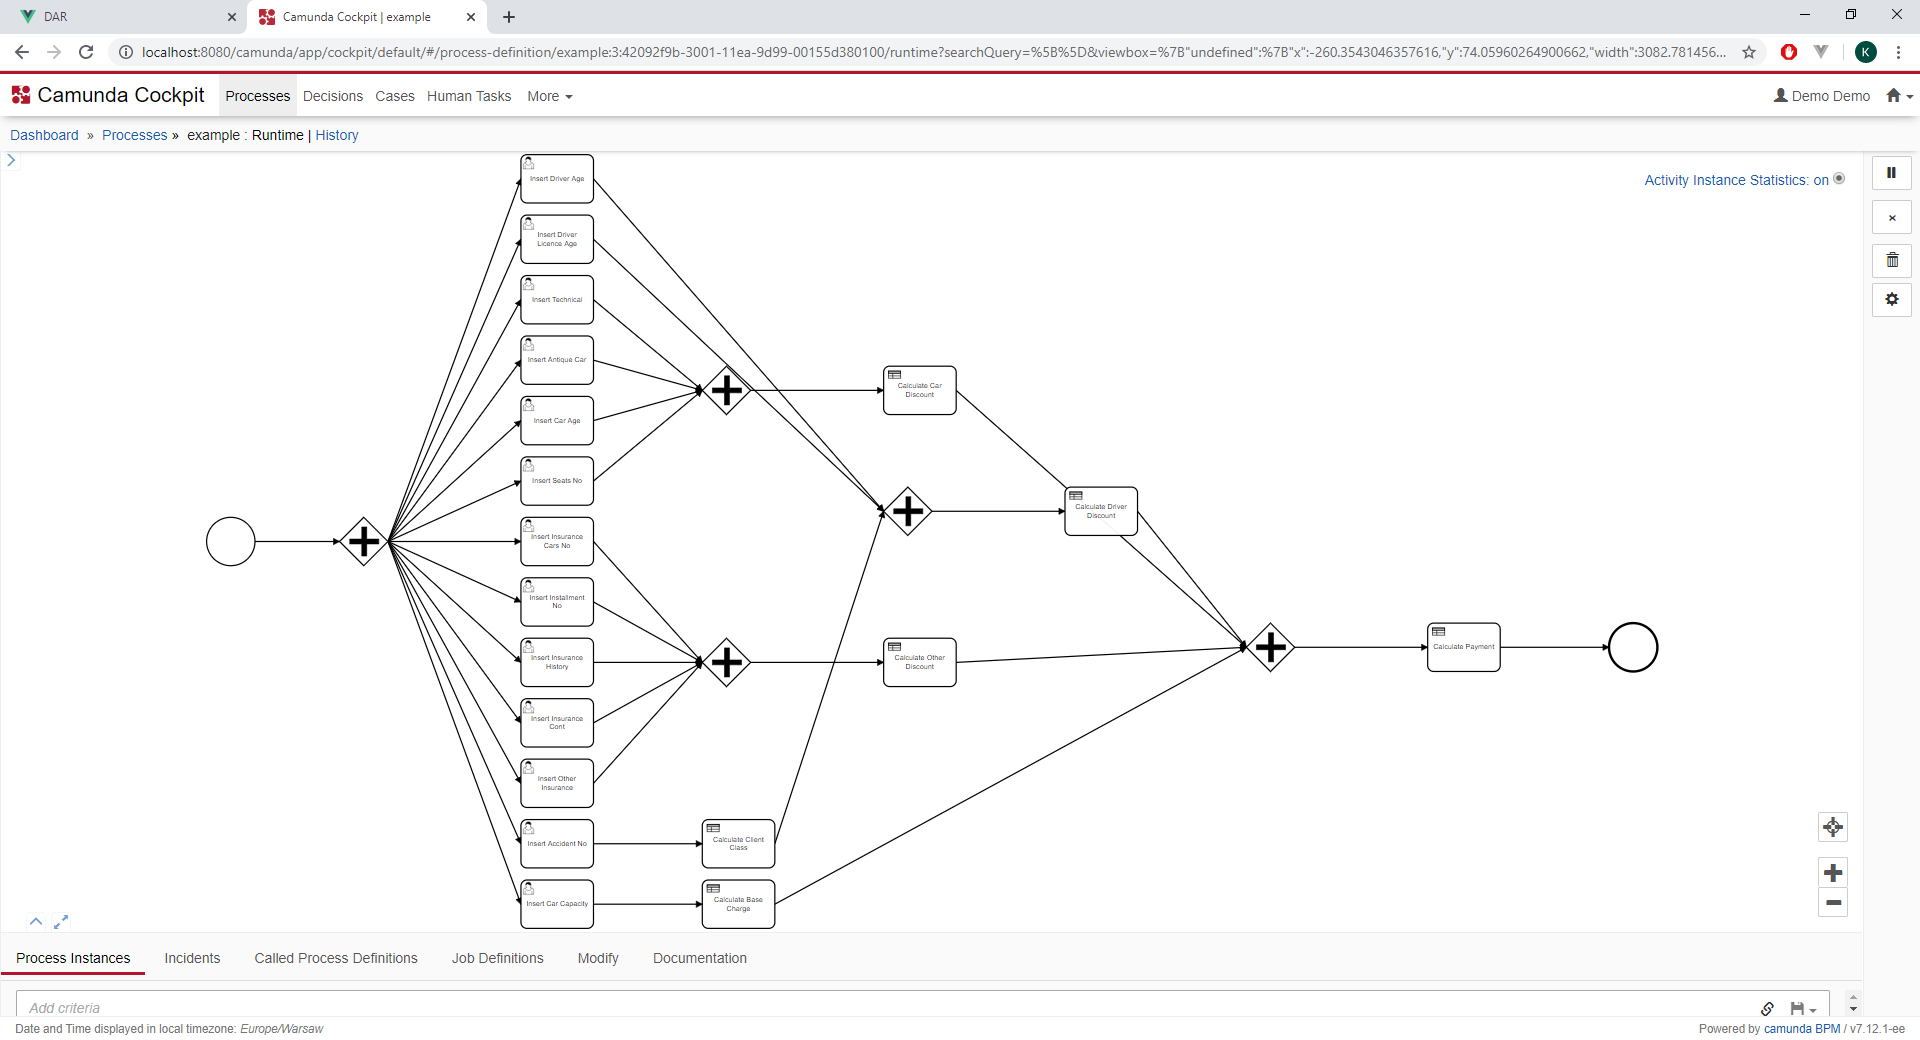
\includegraphics[width=\textwidth]{./assets/camundaExampleBPMN.png}
    \caption{Model \emph{BPMN} pliku ,,example''}
    \label{fig:camundaExampleBPMN}
\end{figure}
\begin{figure}
    \centering
    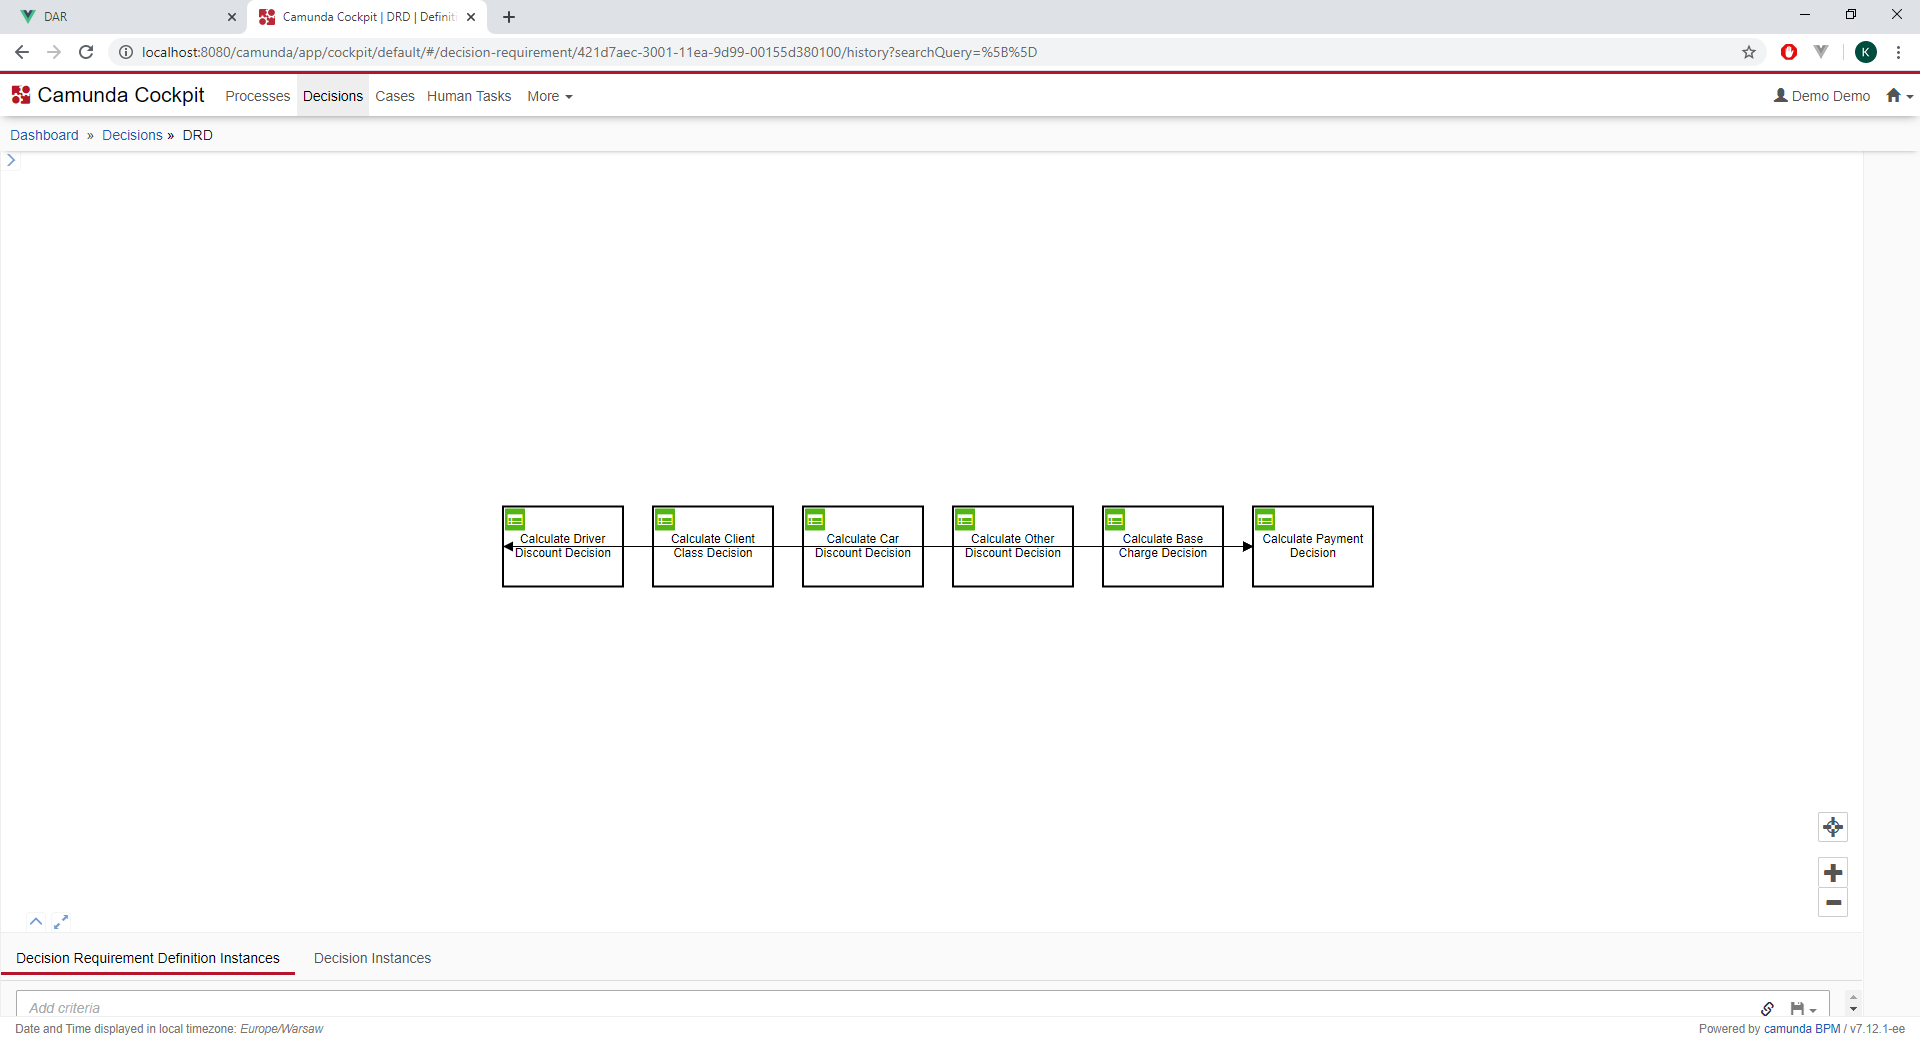
\includegraphics[width=\textwidth]{./assets/camundaExampleDMN.png}
    \caption{Model \emph{DMN} pliku ,,example''}
    \label{fig:camundaExampleDMN}
\end{figure}

Jak już zostało w~pracy nadmienione diagramy \emph{ARD} dostarczają informacje pozwalające na stworzenie modeli \emph{DMN} oraz związanych z~nimi tablic decyzyjnych, w~których określona jest ilość atrybutów wejściowych i~wyjściowych, ich nazwy oraz typy wartości. Reguły biznesowe jednak pozostają puste. Dlatego po wdrożeniu użytkownik musi sam edytować tablice decyzyjne i~według własnego uznania wypełnić reguły. Rysunek~\ref{fig:camundaExampleRules} prezentuje edycję jednej z~tablic decyzyjnych związanych z~jedną z~decyzji z~rysunku~\ref{fig:camundaExampleDMN}. Na potrzeby przykładu dodane zostały dwa wiersze reguł. Każda z~tablic decyzyjnych została w~podobny sposób wypełniona, aby móc uruchomić proces.
\begin{figure}
    \centering
    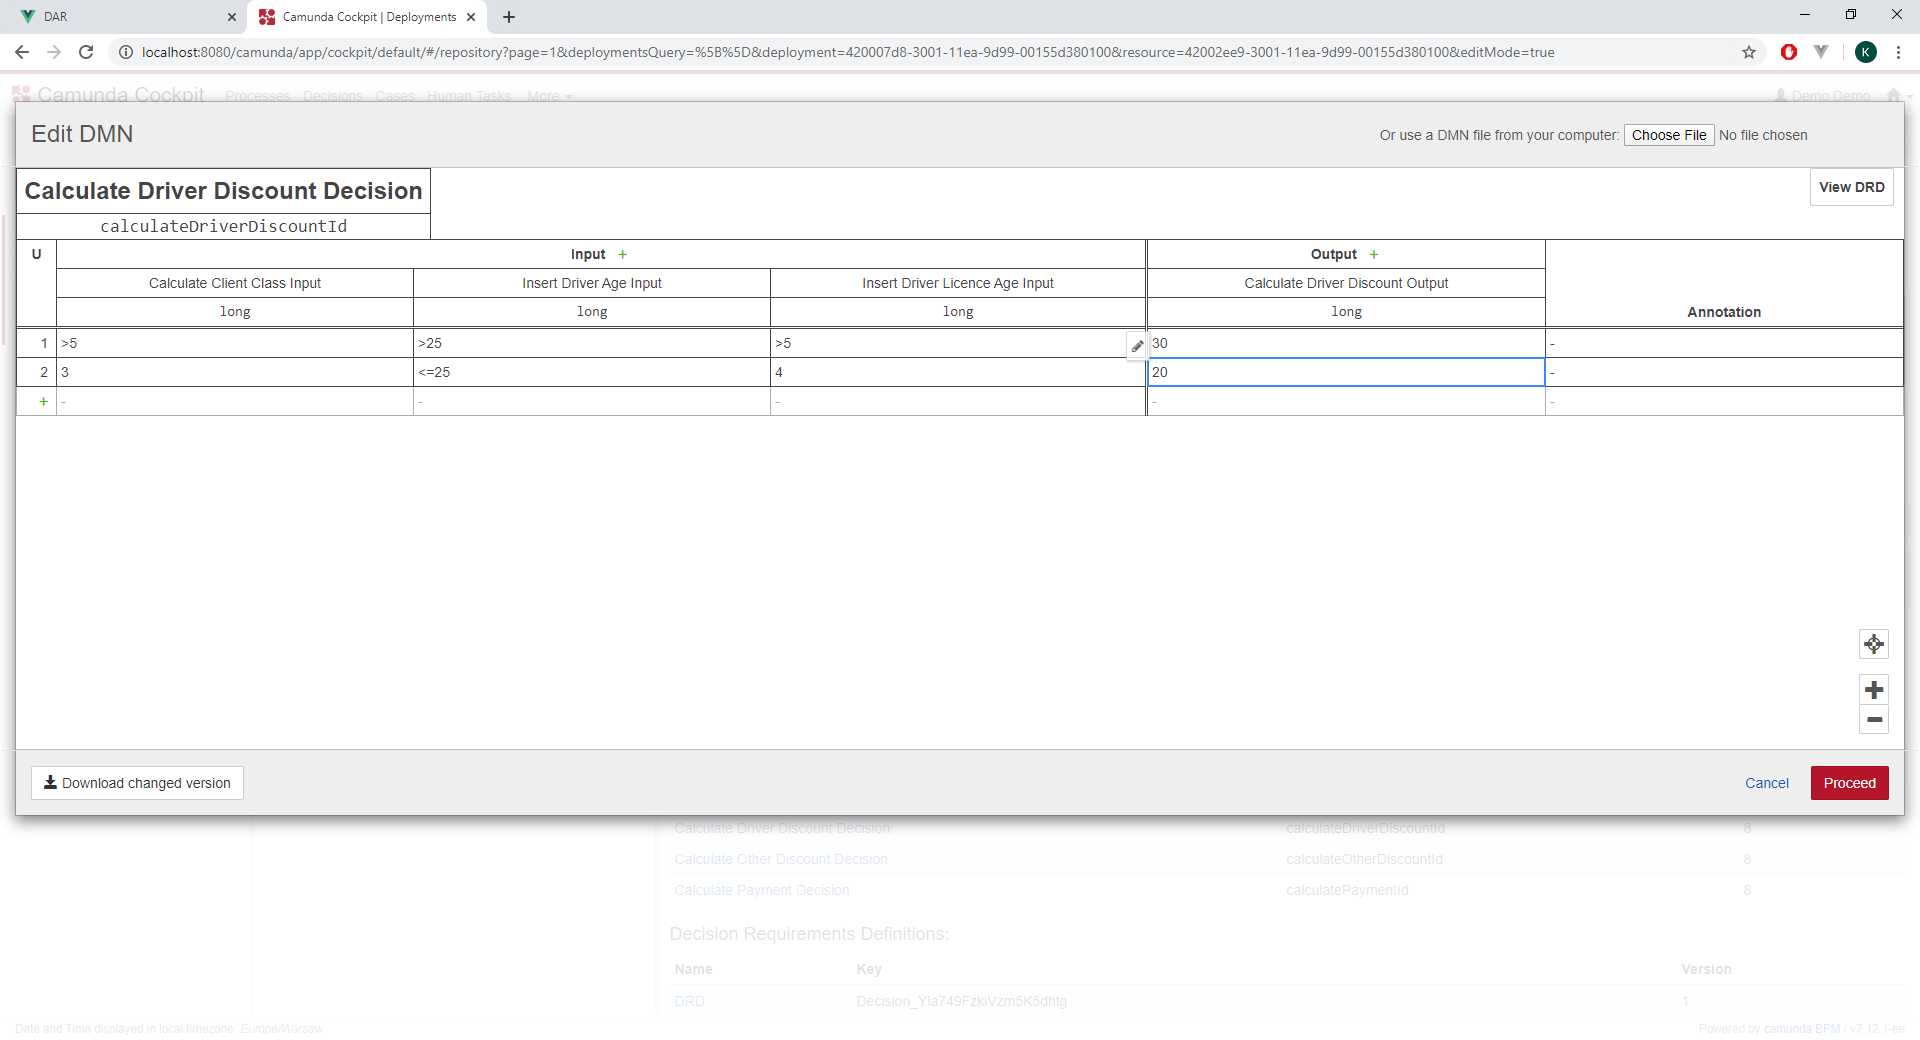
\includegraphics[width=\textwidth]{./assets/camundaExampleRules.png}
    \caption{Edycja tablicy decyzyjnej}
    \label{fig:camundaExampleRules}
\end{figure}

W tym momencie nic nie stoi na przeszkodzie, aby uruchomić proces. Żeby tego dokonać trzeba przejść do \emph{Camunda Tasklist} (używając menu, w~prawym górnym rogu interfejsu w~kształcie domku). Widok z~jakim spotyka się użytkownik jest przedstawiony na rysunku~\ref{fig:camundaTasklistDefault}. Tutaj wyświetlone będą wszystkie zadania wykonywalne przez użytkownika potrzebne do działania procesu, np. zadania związane z~podaniem danych wejściowych. Wyświetlone zadania można odpowiednio filtrować.
\begin{figure}
    \centering
    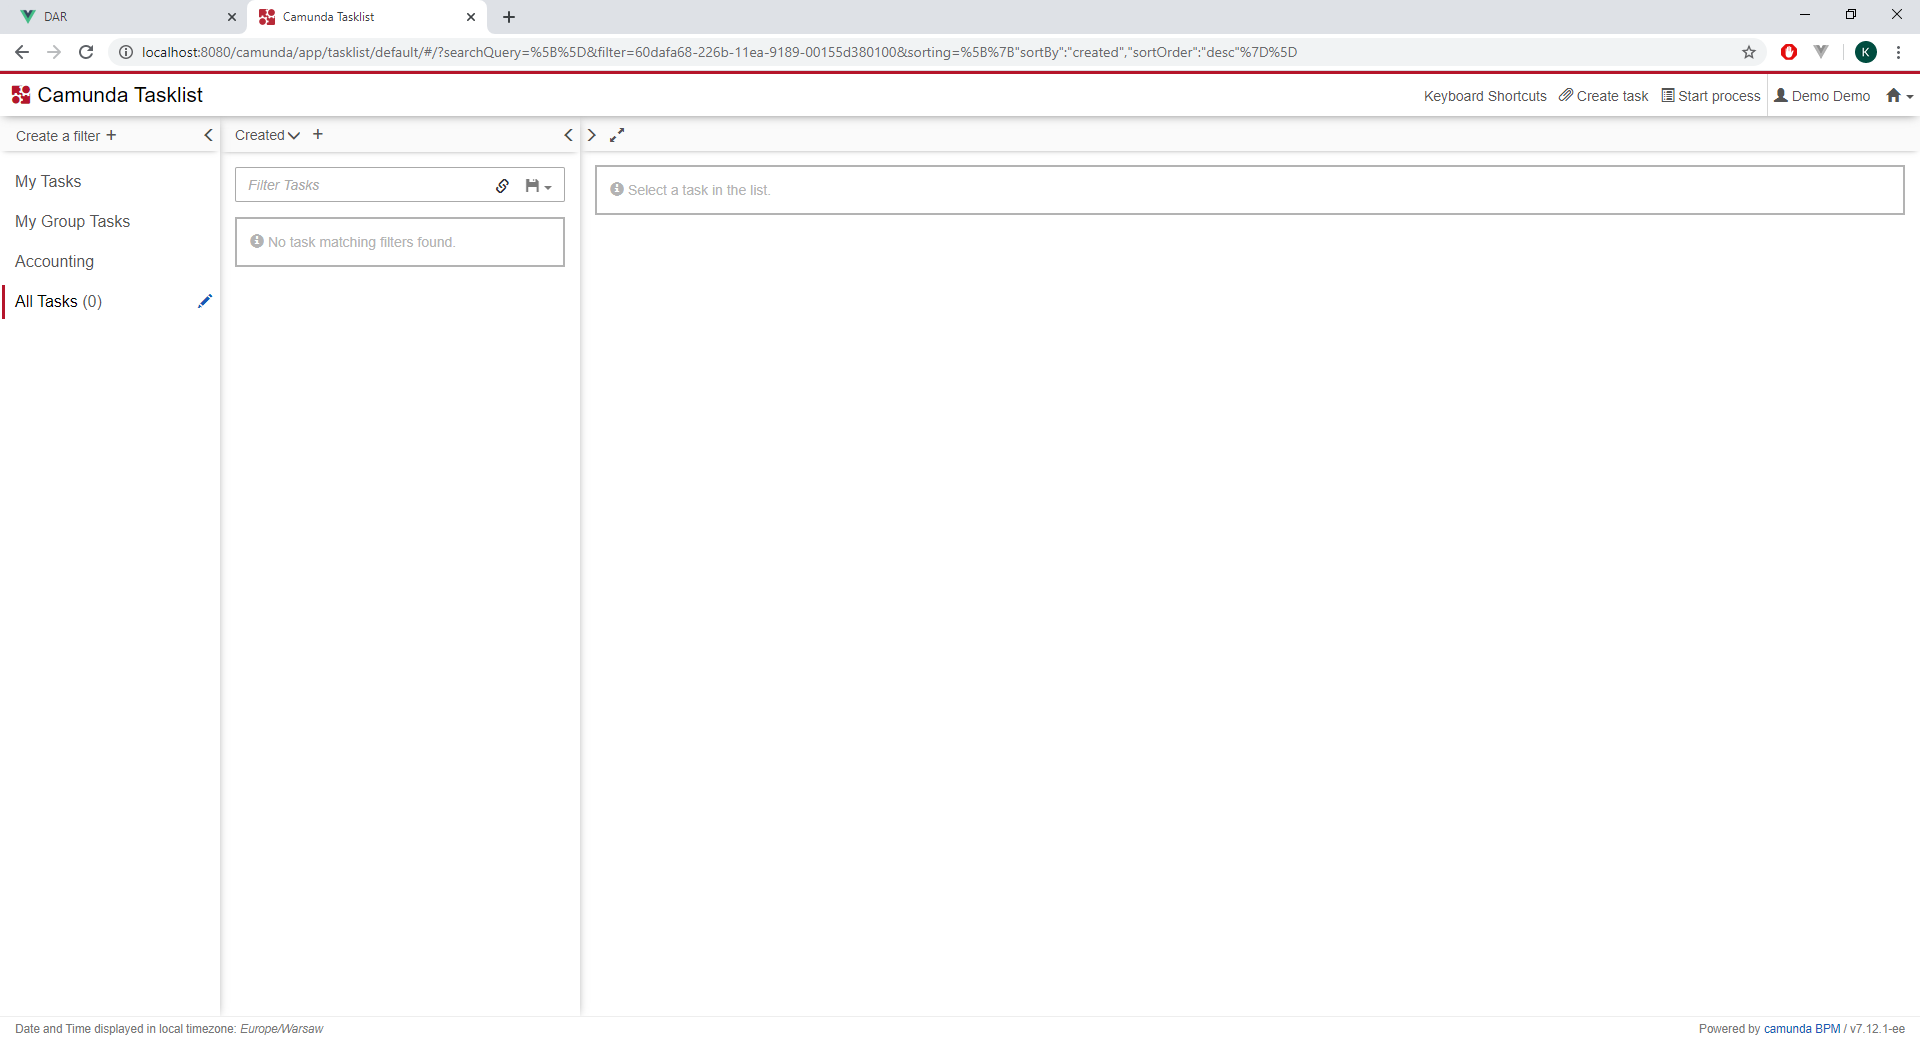
\includegraphics[width=\textwidth]{./assets/camundaTasklistDefault.png}
    \caption{Domyślny ekran \emph{Camunda Tasklist}}
    \label{fig:camundaTasklistDefault}
\end{figure}

Aby uruchomić proces, należy wybrać przycisk ,,Start process'' w~prawym górnym rogu, wybrać odpowiedni model \emph{BPMN} (w~tym przypadku będzie to ,,example''), nadać tej instancji procesu pewien identyfikator, dla przykładu będzie to ,,ExampleBuisnessKey'' i~nacisnąć przycisk ,,Start''. Spowoduje to pojawienie się adnotacji, że proces został uruchomiony. Można w~tym momencie wrócić do modułu \emph{Camunda Cockpit}, gdzie na stronie z~rysunku~\ref{fig:camundaCockpitDefault} w~metrykach nastąpi zmiana -- pokazane zostanie, że pewien proces działa. W zakładce ,,Processes'' wyświetlona będzie instancja procesu, która po naciśnięciu pokaże aktualny stan wykonywania procesu. Jednak przed przejściem do wspomnianego modułu warto odświeżyć \emph{Camunda Tasklist}. Pojawi się lista wykonywalnych zadań związanych z~procesem, który został uruchomiony. Są to dane wejściowe, które musi podać użytkownik, aby proces kontynuować działanie. Rysunek~\ref{fig:camundaTasklistTask} prezentuje opisaną listę oraz wypełnienie jednego z~takich zadań. Na potrzeby przykładu wszystkie zadania zostały wykonane.
\begin{figure}
    \centering
    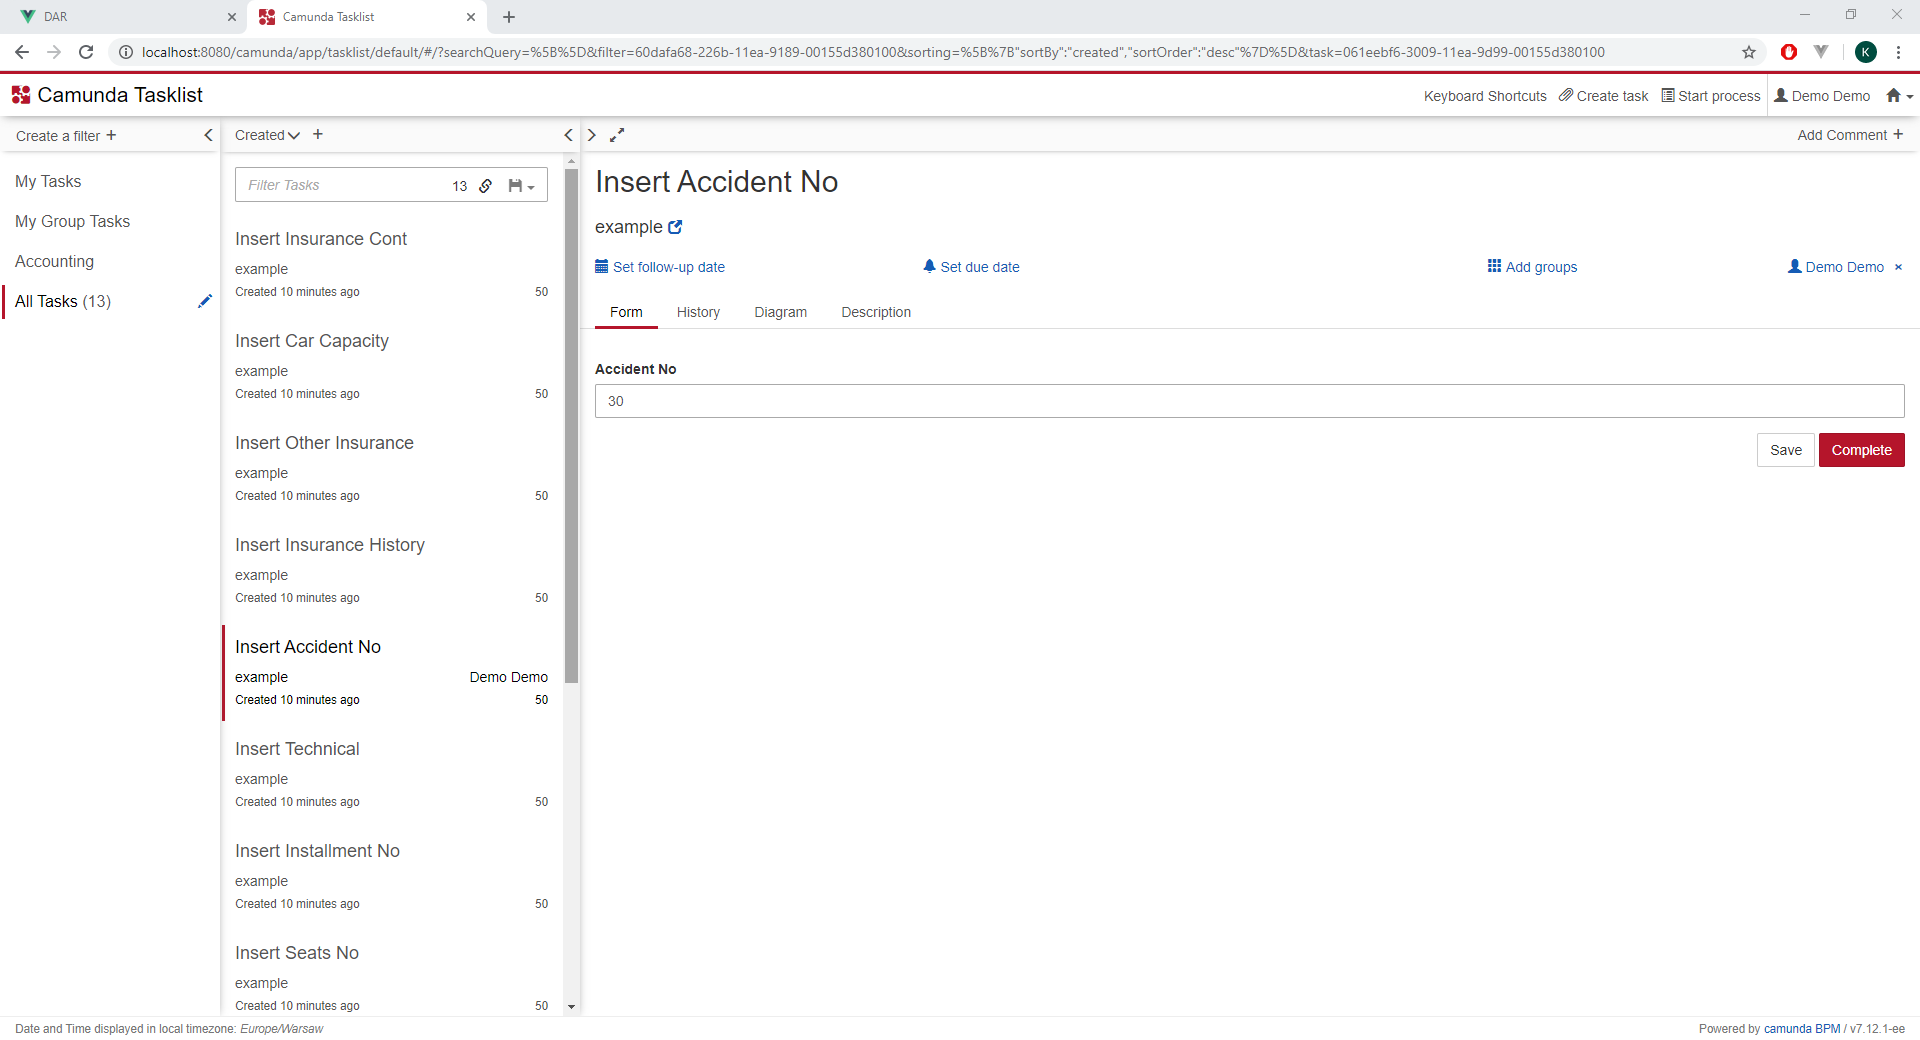
\includegraphics[width=\textwidth]{./assets/camundaTasklistTask.png}
    \caption{Wypełnione \emph{zadanie} wraz z~listą oczekujących zadań}
    \label{fig:camundaTasklistTask}
\end{figure}

Po wykonaniu wszystkich zadań warto przejść do modułu \emph{Camunda Cockpit} do zakładki ,,Processes'', wybrać tam odpowiedni proces i~po wyświetleniu modelu \emph{BPMN} nacisnąć przycisk ,,History''. Opcja ,,Runtime'' w~tym momencie nic nie wyświetla, ponieważ proces został zakończony, wszystkie decyzje zostały zewaluowane, jednak tak jak to było opisywane wcześniej, w~przypadku wykonywania procesu to jest miejsce, gdzie można śledzić działanie procesu. Rysunek~\ref{fig:camundaCockpitCompleted} prezentuje widok ,,History''. 
\begin{figure}
    \centering
    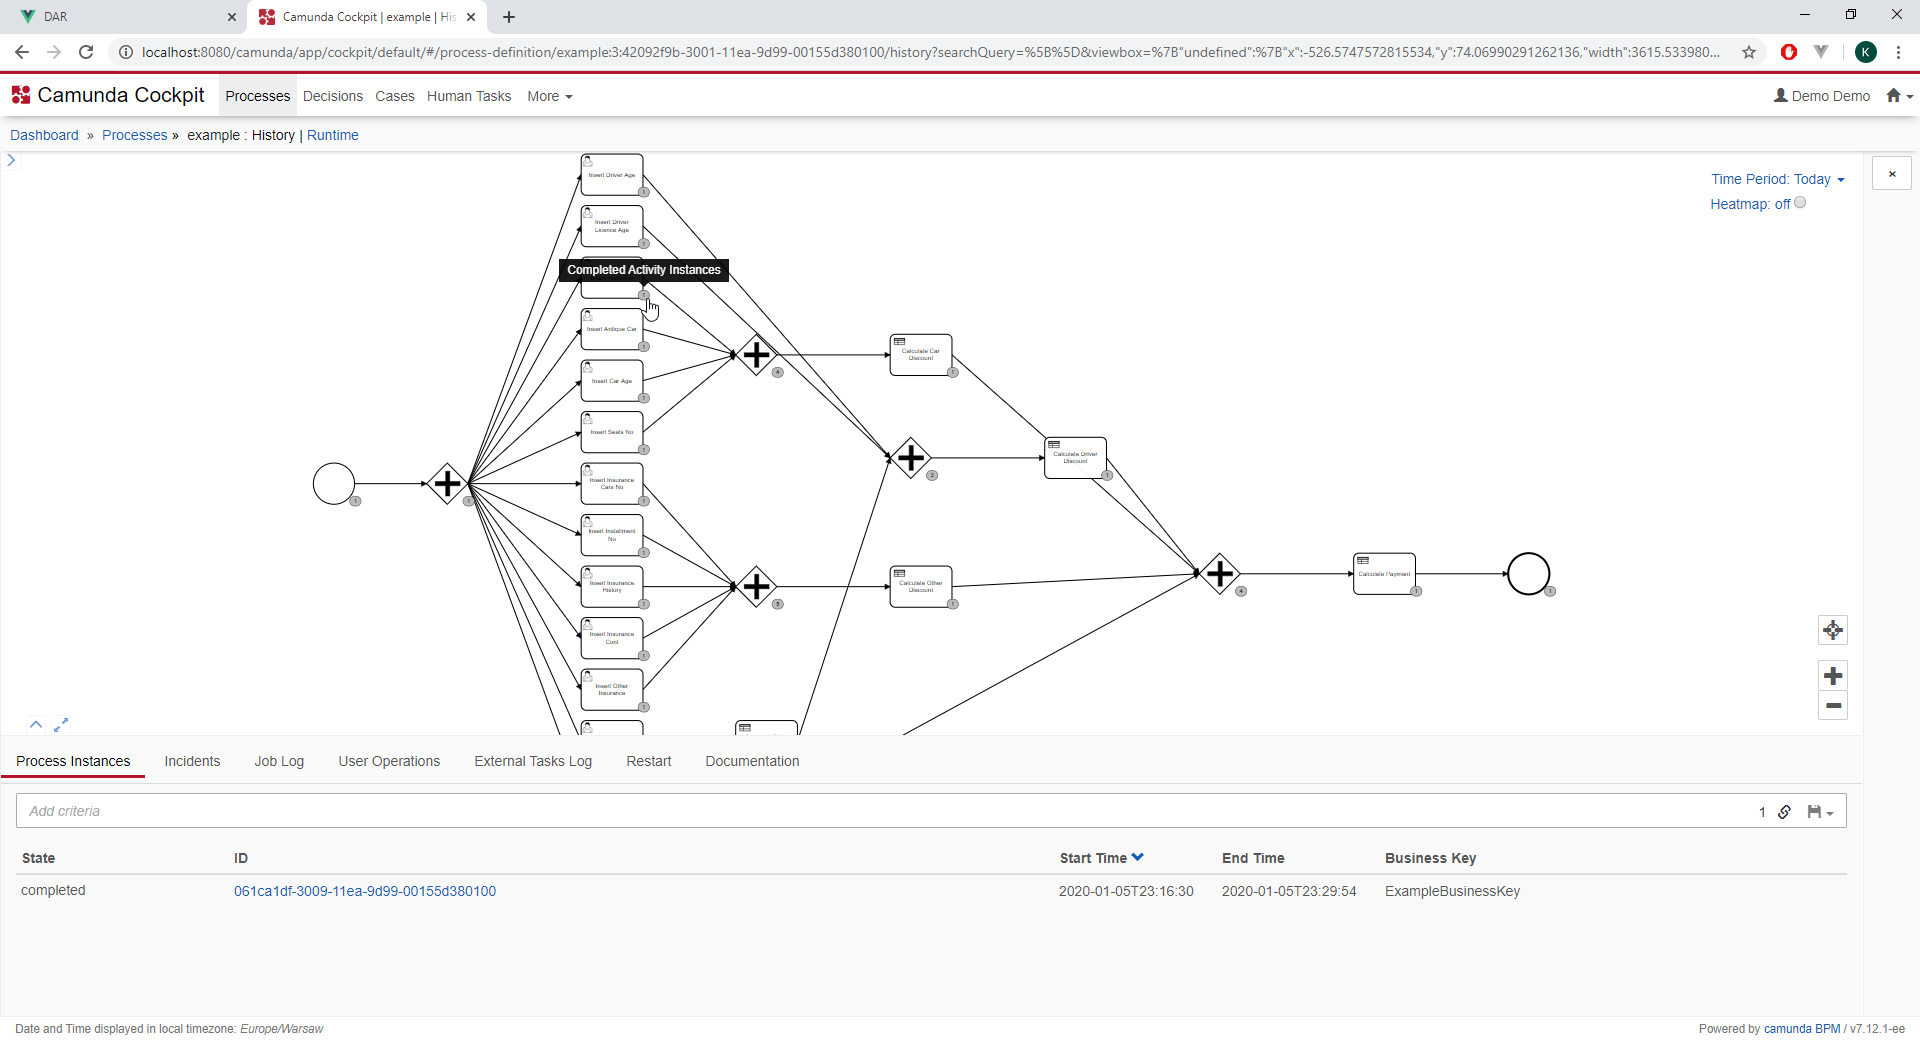
\includegraphics[width=\textwidth]{./assets/camundaCockpitCompleted.png}
    \caption{Historia wykonywania procesu}
    \label{fig:camundaCockpitCompleted}
\end{figure}
Dodatkowo można w~tym miejscu sprawdzić jak rozkładała się praca procesu, aby ewentualnie go usprawniać. Rysunek~\ref{fig:camundaCockpitHeat} przedstawia przydatny do tego widok.
\begin{figure}
    \centering
    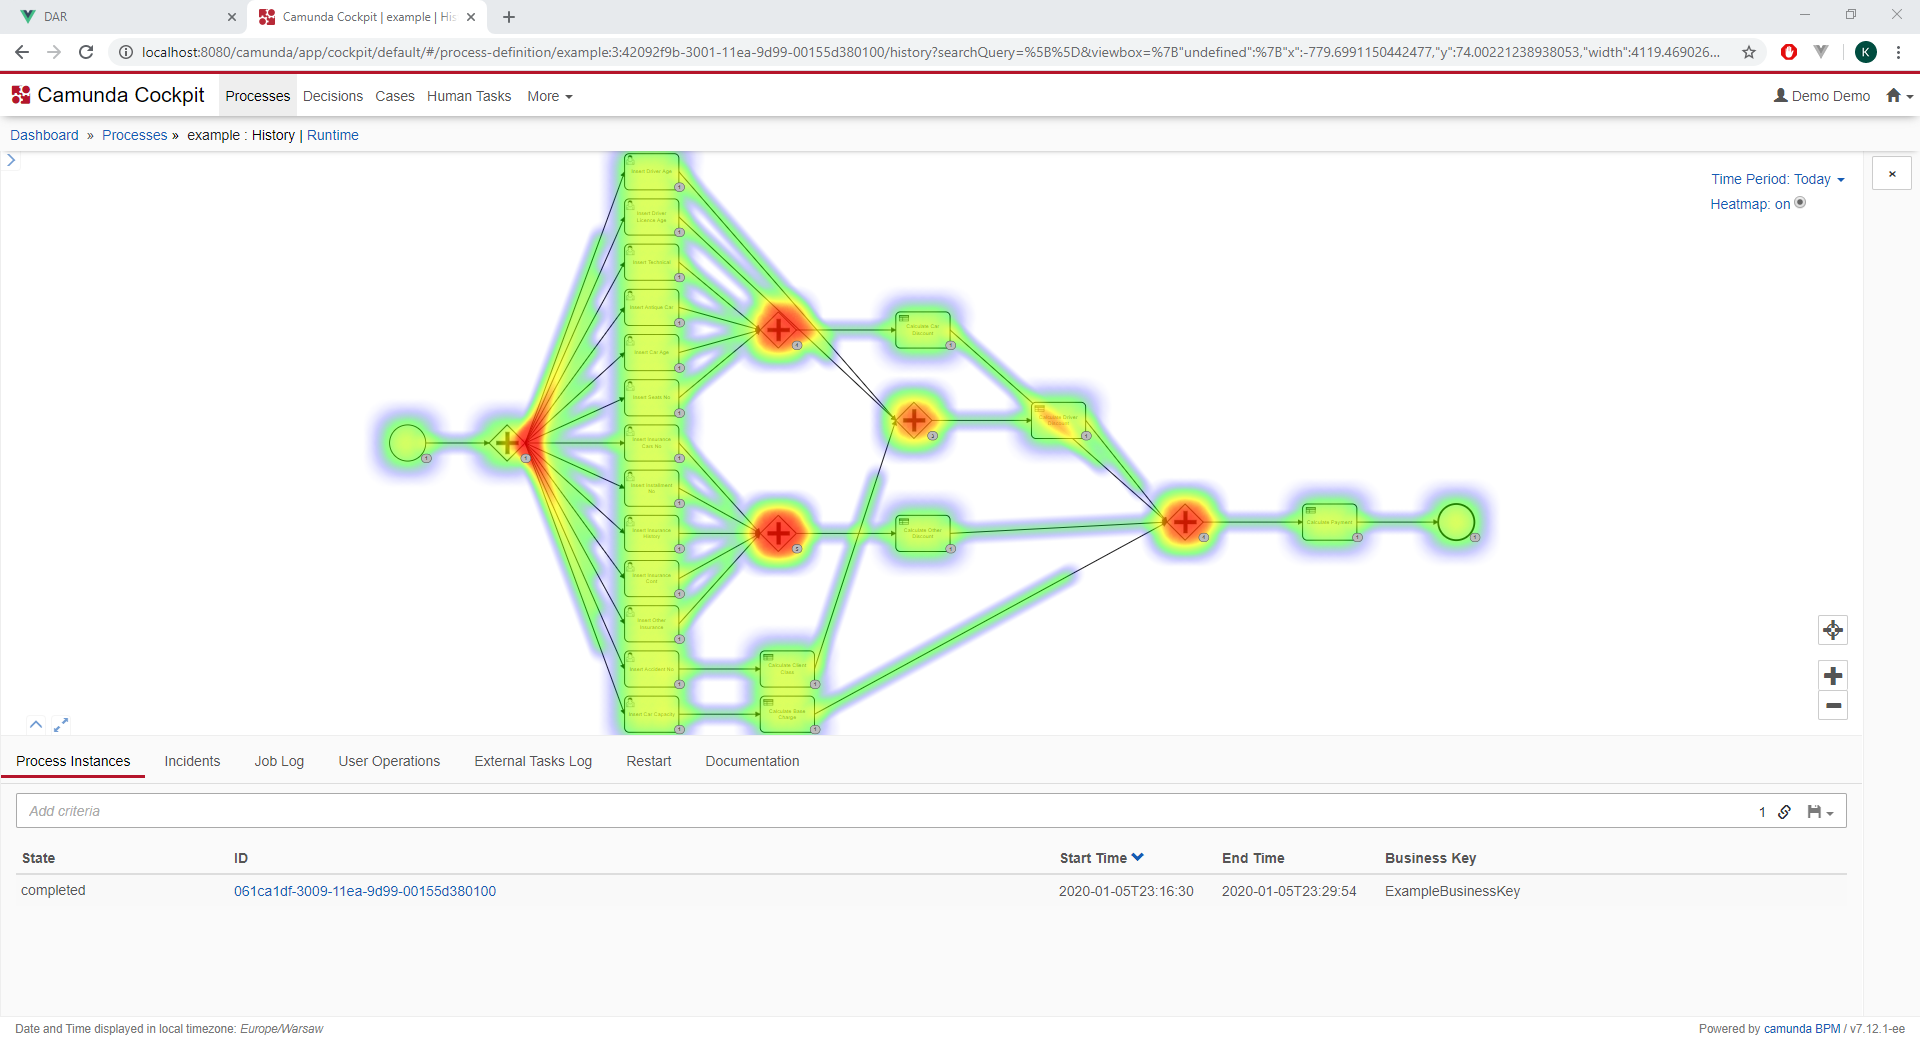
\includegraphics[width=\textwidth]{./assets/camundaCockpitHeat.png}
    \caption{Rozkład pracy procesu}
    \label{fig:camundaCockpitHeat}
\end{figure} 

W dolnej części rysunku~\ref{fig:camundaCockpitCompleted} widać instancję zakończonego procesu. Po naciśnięciu ,,ID'' tej instancji, widok modelu zostaje ten sam, jednak dochodzi wiele zakładek związanych z~historią wykonywania tego procesu, np. jakie zadania zostały wykonane, jakie były wartości danych i~jakie decyzje zostały ewaluowane. Aby zobaczyć wynik końcowy wystarczy przejść do ewaluowanych decyzji i~wybrać finalną decyzję, czyli w~prezentowanym przykładzie ,,Calculate Payment''. Po wybraniu tej decyzji zostaje tylko przejść do jej instancji. Rysunek~\ref{fig:camundaCockpitFinal} przedstawia wynik całego procesu i~jakie były finalne wartości atrybutów -- koszt ubezpieczenia w~tym przypadku wyniósł 100 PLN. Oczywiście w~ramach przykładu reguły są trywialne, w~przedstawionej tablicy decyzyjnej występuje tylko jeden wiersz reguł, jednak w~prawdziwym świecie może ich być dowolna liczba.
\begin{figure}
    \centering
    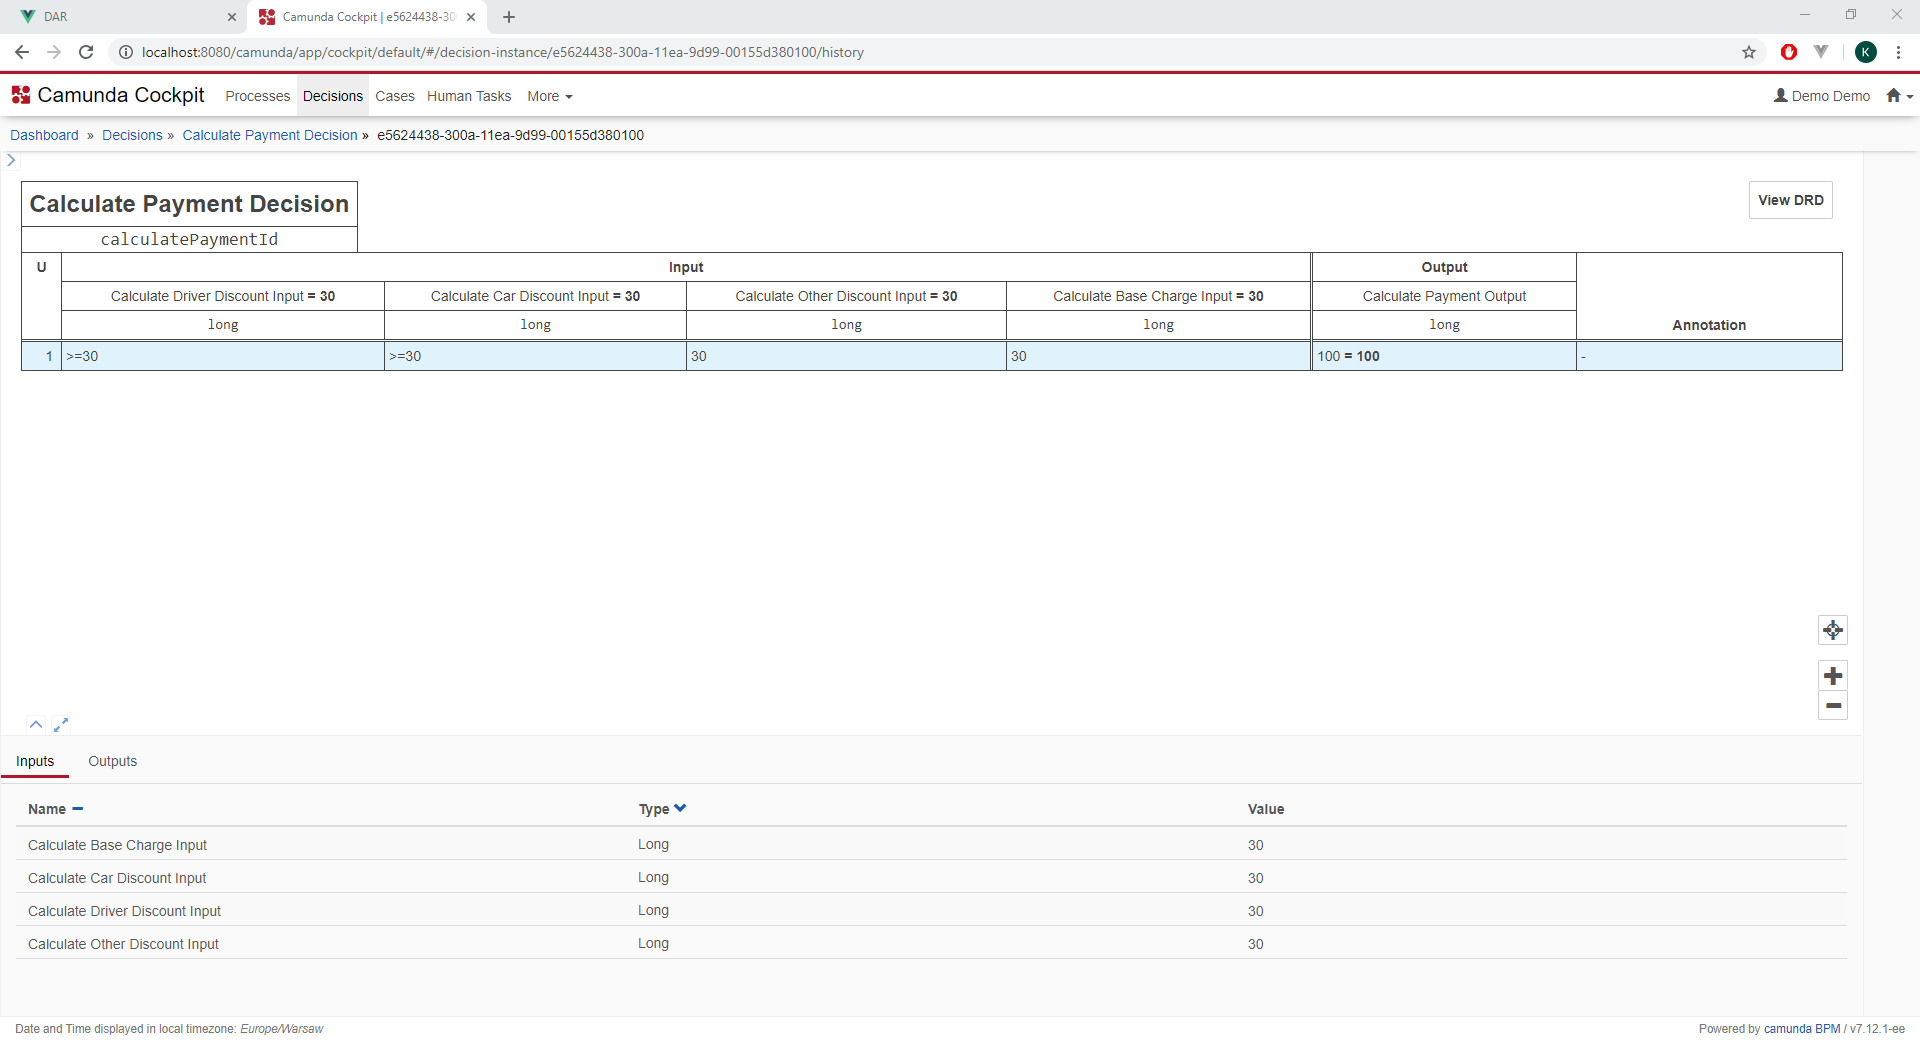
\includegraphics[width=\textwidth]{./assets/camundaCockpitFinal.png}
    \caption{Wynik procesu}
    \label{fig:camundaCockpitFinal}
\end{figure}
\vspace{-6mm}
%---------------------------------------------------------------------------
\section{Podsumowanie wyników}
\label{sec:podsumowanieWyników}
Aplikacja spełnia wszystkie założone wymagania. Generowane modele w~notacji \emph{BPMN} oraz \emph{DMN} poprawnie opisują diagram \emph{ARD} zapisany w~podanym pliku \emph{HML}. Interfejs aplikacji ,,DAR`` jest intuicyjny i~przejrzysty. Kod aplikacji w~większości jest asynchroniczny co sprawia, że aplikacja jest płynniejsza w~działaniu. Zintegrowany system \emph{Camunda} poprawnie uruchamia wdrożone procesy. W~przypadku decyzji, ewaluacja również jest poprawna, wymogiem jest tylko uzupełnienie reguł przez użytkownika. Sam wynik końcowy jest zadowalający i~zgodny z~oczekiwaniami.
\vspace{4mm}

Jest to koniec rozdziału przedstawiającego działanie aplikacji. W tym rozdziale przedstawione zostały najważniejsze funkcjonalności systemu na konkretnym przykładzie. W kolejnym, końcowym rozdziale przedstawione zostaną wnioski nasuwające się po zapoznaniu się z~aplikacją oraz możliwe kierunki rozwoju aplikacji. 


